              
%%%%%%%%%%%%%%%%%%%%%%%%%%%%%%%%%%%%%%%%%
% Journal Article
% LaTeX Template
% Version 1.3 (9/9/13)
%
% This template has been downloaded from:
% http://www.LaTeXTemplates.com
%
% Original author:
% Frits Wenneker (http://www.howtotex.com)
%
% License:
% CC BY-NC-SA 3.0 (http://creativecommons.org/licenses/by-nc-sa/3.0/)
%
%%%%%%%%%%%%%%%%%%%%%%%%%%%%%%%%%%%%%%%%%
%----------------------------------------------------------------------------------------
%       PACKAGES AND OTHER DOCUMENT CONFIGURATIONS
%----------------------------------------------------------------------------------------
\documentclass[paper=letter, fontsize=12pt,spanish]{article}
\usepackage[spanish]{babel} % English language/hyphenation
\usepackage{amsmath,amsfonts,amsthm} % Math packages
\usepackage[utf8]{inputenc}
\usepackage{float}
\usepackage{lipsum} % Package to generate dummy text throughout this template
\usepackage{blindtext}
\usepackage{graphicx} 
\usepackage{caption}
\usepackage{subcaption}
\usepackage[sc]{mathpazo} % Use the Palatino font
\usepackage[T1]{fontenc} % Use 8-bit encoding that has 256 glyphs
\linespread{1.05} % Line spacing - Palatino needs more space between lines
\usepackage{microtype} % Slightly tweak font spacing for aesthetics
\usepackage[hmarginratio=1:1,top=32mm,columnsep=20pt]{geometry} % Document margins
\usepackage{multicol} % Used for the two-column layout of the document
%\usepackage[hang, small,labelfont=bf,up,textfont=it,up]{caption} % Custom captions under/above floats in tables or figures
\usepackage{booktabs} % Horizontal rules in tables
\usepackage{float} % Required for tables and figures in the multi-column environment - they need to be placed in specific locations with the [H] (e.g. \begin{table}[H])
\usepackage{hyperref} % For hyperlinks in the PDF
\usepackage{lettrine} % The lettrine is the first enlarged letter at the beginning of the text
\usepackage{paralist} % Used for the compactitem environment which makes bullet points with less space between them
\usepackage{abstract} % Allows abstract customization
\renewcommand{\abstractnamefont}{\normalfont\bfseries} % Set the "Abstract" text to bold
\renewcommand{\abstracttextfont}{\normalfont\small\itshape} % Set the abstract itself to small italic text
\usepackage{titlesec} % Allows customization of titles

\renewcommand\thesection{\Roman{section}} % Roman numerals for the sections
\renewcommand\thesubsection{\Roman{subsection}} % Roman numerals for subsections

\titleformat{\section}[block]{\large\scshape\centering}{\thesection.}{1em}{} % Change the look of the section titles
\titleformat{\subsection}[block]{\large}{\thesubsection.}{1em}{} % Change the look of the section titles
\newcommand{\horrule}[1]{\rule{\linewidth}{#1}} % Create horizontal rule command with 1 argument of height
\usepackage{fancyhdr} % Headers and footers
\pagestyle{fancy} % All pages have headers and footers
\fancyhead{} % Blank out the default header
\fancyfoot{} % Blank out the default footer

\selectlanguage{spanish}

\fancyhead[C]{Programación Fortran $\bullet$ Práctica 7 } % Custom header text

\fancyfoot[RO,LE]{\thepage} % Custom footer text
%----------------------------------------------------------------------------------------
%       TITLE SECTION
%----------------------------------------------------------------------------------------

\title{\vspace{-15mm}\fontsize{24pt}{10pt}\selectfont\textbf{Análisis de series de tiempo de marea en el manglar El Sargento}} % Article title
\author{
\large
{\textsc{Andrés Rodríguez Mendoza}}\\[2mm]
%\thanks{A thank you or further information}\\ % Your name
%\normalsize \href{mailto:marco.torres.810@gmail.com}{marco.torres.810@gmail.com}\\[2mm] % Your email address
}
\date{}
%----------------------------------------------------------------------------------------
\begin{document}
\maketitle % Insert title
\thispagestyle{fancy} % All pages have headers and footers

\graphicspath{{./Graphs/}}

\section{Introducci\'on}
El estudio de las mareas ha sido de gran importancia para el comercio y la ciencia durante cientos de años por diversas razones:
\begin{enumerate}
\item Las mareas pueden producir fuertes corrientes en las aguas costeras, impidiendo la navegación.
\item Las corrientes al mezclarse ayudan a mover la circulación en aguas profundas, influyendo en el clima y en cambios climáticos abruptos.
\item La corteza terreste se dobla bajo la influencia del potencial de marea y por el peso de las aguas oceánicas. Como consecuencia, el suelo del mar y los continentes se mueven arriba y abajo alrededor de 10 cm respondiendo a la marea.
\item Las mareas oceánicas producen fuerzas que transfieren momento angular entre la Tierra y el cuerpo que genera la marea, especialmente la Luna. Como resultado de las fuerzas de marea, la rotación de la Tierra sobre su eje se ralentiza, incrementando la duración del día; la rotación de la Luna sobre la Tierra se ralentiza; y la rotación de la Luna sobre su eje también ralentiza, causando a la Luna mantener el mismo lado de su superficie mirando a la Tierra mientras rota alrededor de ella.
\item Las mareas influyen en la órbita de satelites. El conocimiento de las mareas se requiere para el cómputo de la orbita de satélites altimétricos y para corregir mediciones de topografía oceánica.
\end{enumerate}

Desde hace siglos es sabido que las mareas estan relacionadas con las fases de la luna. La relación exacta, sin embargo, está oculta detras de complicados factores, y algunos de las más grandes mentes científicas de los últimos cuatro siglos trabajaron para entender, calcular, y predecir las mareas. Galileo, Descartes, Kepler, Newton, Euler, Bernoulli, Laplace y muchos otros contribuyeron a esto. Algunas de las primeras computadoras fueron desarrolladas para calcular y predecir mareas. 

Las mareas son calculadas de las ecuaciones de hidrodinámica para un cuerpo océanico autogravitante sobre tierra elástica rotando. La fuerza motriz es el gradiente del campo gravitacional de la Luna y el Sol. Si la Tierra fuera un planeta de océano sin tierra, y se ingorara la influencia de la incercia y corrientes, los gradientes de gravedad producirian un par de protuberancias de agua sobre la tierra, una del lado volteando hacia la Luna o al Sol, y la otra del lado opuesto.

Los cambios en el nivel del agua es resultado de una superposición diversos factores denominados constituyentes de marea, los cuales determinan las frecuencias fundamentales de la marea.
Para calcular la amplitud y la fase de la marea en un océano, se calculan los potenciales que generan las mareas provenientes del Sol y la Luna. De los potenciales se puede separar el periodo del potencial de marea lunar en tres términos de alrededor de 14 dias, 24 horas, y 12 horas. Similarmente el potencial del Sol tiene periodos cerca de 180 dias, 24 horas, y 12 horas. Así, quedan 6 distintos grupos de frecuencias de marea.
Con una expansion de Doodson se puede descomponer los constituyentes de marea en grupos con frecuencias similares. Cada constituyente tiene una frecuencia 

\begin{equation}
\label{eq1}
f = n_1 f_1 + n_2 f_2 + n_3 f_3 + n_4 f_4 + n_5 f_5 + n_6 f_6, 
\end{equation}


\begin{table}
\centering 
\begin{tabular}{l l l }
\toprule
     & 	Periodo  	& Fuente\\
\midrule
$f_1$&	d\'ia lunar	& Tiempo medio lunar local\\
$f_2$&	mes		& Longitud lunar media\\
$f_3$& año	& Longitud solar media\\
$f_4$&	años	& Longitud de perigeo lunar\\
$f_5$& años & Longitud del nodo ascendente lunar\\
$f_6$& años & Longitud del perigeo solar\\
\bottomrule 

 \end{tabular}
\caption {Frecuencias fundamentales} \label{tab:title} 
\end{table}

donde los entero $n_i$ son los numeros de Doodson, a veces llamados una marea parcial. $n_1 = 1,2,3$ y $n_2-n_6$ están entre -5 y 5. Los números de Doodson $n_6$ usualmente se ignoran porque la modulación de largo término de las mareas por el cambio en el perigeo del Sol es muy pequeña.



\begin{table}[ht!]
\centering 

\begin{tabular}{l c l l l l l r}
\toprule
Tipo de Marea & Nombre & $n_1$ & $n_2$ & $n_3$ & $n_4$ & $n_5$ & Periodo (hr)\\
\midrule
Semidiurna & & & & & & & \\ \\
Lunar principal & $M_2$ & 2 & 0 & 0 & 0 & 0 & 12.4206\\
Solar principal & $S_2$ & 2 & 2 & -2 & 0 & 0 & 12.0000\\
Elíptica lunar & $N_2$ & 2 & -1 & 0 & 1 & 0 & 12.6584\\
Lunisolar & $K_2$ & 2 & 2 & 0 & 0 & 0 & 11.9673\\
\midrule
Diurna & & & & & & &\\ \\
Lunisolar & $K_1$ & 1 & 1 & 0 & 0 & 0 & 23.9344\\
Lunar principal & $O_1$ & 1 & -1 & 0 & 0 & 0 & 25.8194\\
Solar principal & $P_1$ & 1 & 1 & -2 & 0 & 0 & 24.0659\\
Lunar elíptica & $Q_1$ & 1 & -2 & 0 & 1 & 0 & 26.8684 \\
\midrule
Periodo largo & & & & & & & \\ \\ 
Quincenal & $M_f$ & 0 & 2 & 0 & 0 & 0 & 327.85\\
Mensual & $M_m$ & 0 & 1 & 0 & -1 & 0 & 661.31 \\
Semianual & $S_sa$ & 0 & 0 & 2 & 0 & 0 & 4383.05 \\
      
\bottomrule 

 \end{tabular}
\caption {Constituyentes de marea} \label{tab:title} 
\end{table}

\section{Resulados}
De los datos proporcionados sobre el manglar El Sargento se calcularon los periodos medios en que ocurren máximos cada mes, cada día y cada mitad de día. Los resultados se muestran en la tabla 3 expresados en días y en horas. Se puede observar la semejanza en la periodicidad de cada marea con los datos sobre los constituyentes.

\begin{table}[ht!]
\centering 
\begin{tabular}{l l l}
\toprule

           Tipo de marea & Periodo (días)  &  Periodo (Hrs)  \\ \midrule
		   Periodo Largo & 26.704 & 640.90 \\         
           Diurno & 0.996 & 23.90 \\ 
           Semidiurno & 0.498 & 11.95 \\
         \bottomrule
        
    \end{tabular}

\caption {Tabla con resultados de periodos} \label{tab:title}  
\end{table}

De la última de las gráficas es de la que se puede obtener mas información. De ahí se concluye que el tipo de marea en el manglar El Sargento es \underline{marea semi-diurna}, debido a que ocurren dos máximos cada día donde su diferencia es menor a un metro, y donde los mínimos varían muy poco.





\section{Gr\'aficas}

\begin{figure}[ht!]
\centering
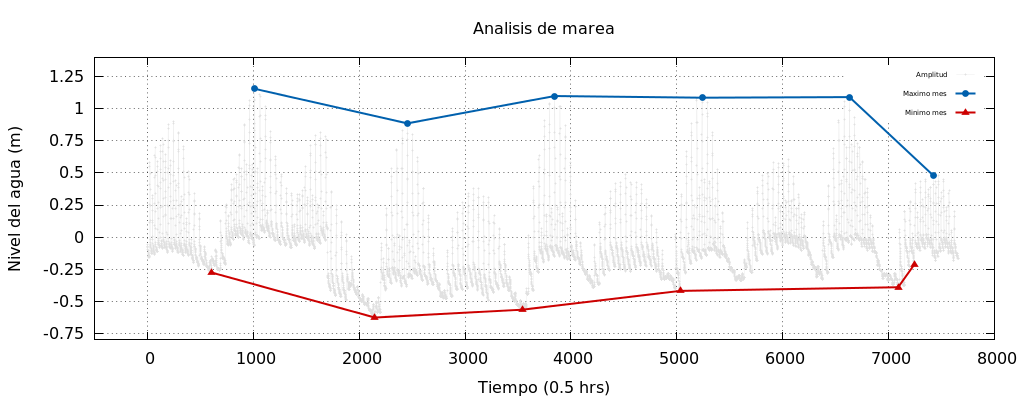
\includegraphics[scale=0.42]{mes}
\caption{M\'aximos y m\'inimos en cada mes}\label{resupsim}
\end{figure}


\begin{figure}[ht!]
\centering
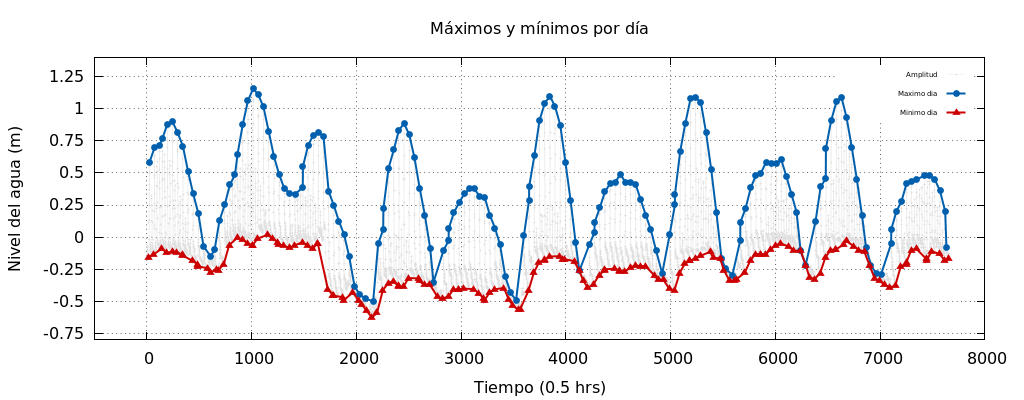
\includegraphics[scale=0.42]{dias}
\caption{M\'aximos y m\'inimos en cada día}\label{resupsim}
\end{figure}


\begin{figure}[ht!]
\centering
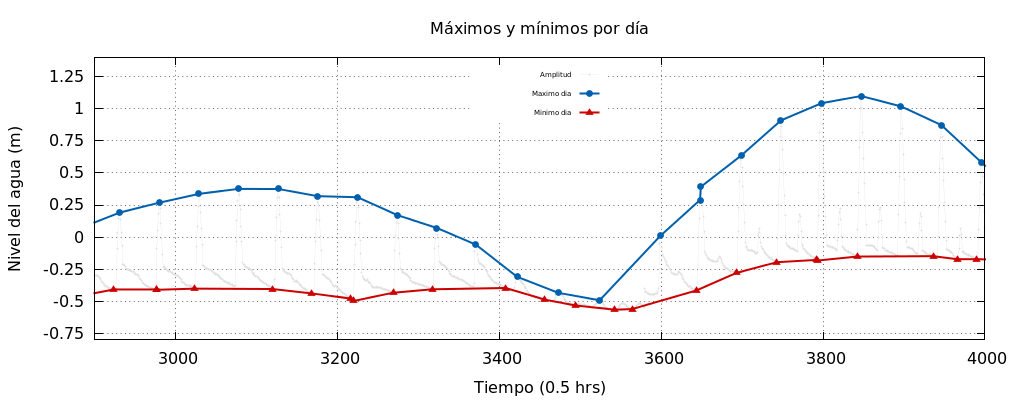
\includegraphics[scale=0.42]{dias2}
\caption{M\'aximos y m\'inimos en cada día (ampliada)}\label{resupsim}
\end{figure}


\begin{figure}[ht!]
\centering
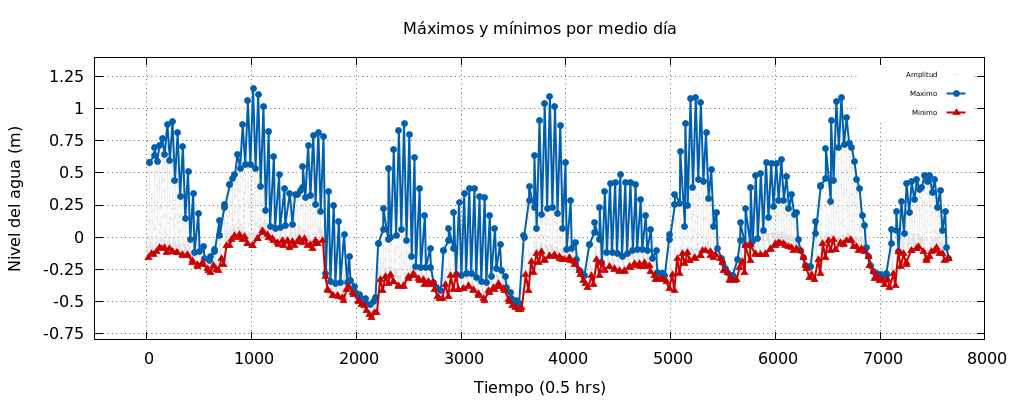
\includegraphics[scale=0.42]{med}
\caption{M\'aximos y m\'inimos en cada mitad de día}\label{resupsim}
\end{figure}

\begin{figure}[ht!]
\centering
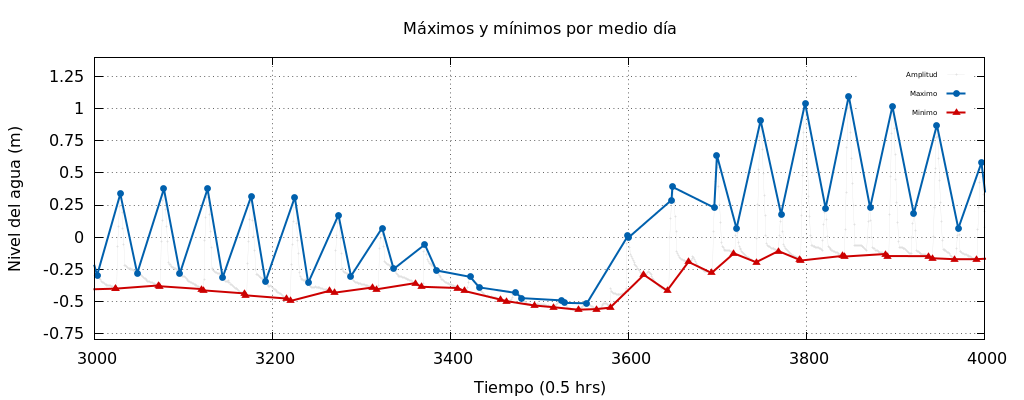
\includegraphics[scale=0.42]{med2}
\caption{M\'aximos y m\'inimos en cada mitad de día (ampliada)}\label{resupsim}
\end{figure}





%----------------------------------------------------------------------------------------
%\end{multicols}
\end{document}
